Image segmentation is a more precise, pixel-level version of object detection. It partitions a digital image into discrete groups of pixels known as image segments, then labels pixels according to their class or instance. \cite{ibm_what_nodate} \\
Depending on the task formulation, segmentation can be divided into:
\begin{itemize}
    \item \textbf{Semantic segmentation}: assigns each pixel in the image to a predefined category, without distinguishing between different object instances belonging to the same class.
    
    \item \textbf{Instance segmentation}: detects and segments each individual object instance in the image, producing a separate mask for each countable object (typically referred to as \emph{things}), while usually not distinguishing amorphous background regions such as sky or ground (\emph{stuff}).
    
    \item \textbf{Panoptic segmentation}: unifies semantic and instance segmentation by providing a complete scene understanding, where both individual object instances (\emph{things}) and uncountable background regions (\emph{stuff}) are segmented in a consistent and non-overlapping manner.\cite{ibm_what_2023}
\end{itemize} 
This fine-grained representation allows for an accurate description of object shapes and boundaries but comes at the cost of higher computational complexity and increased sensitivity to noise and illumination variations.
\begin{figure}[h]
    \centering
    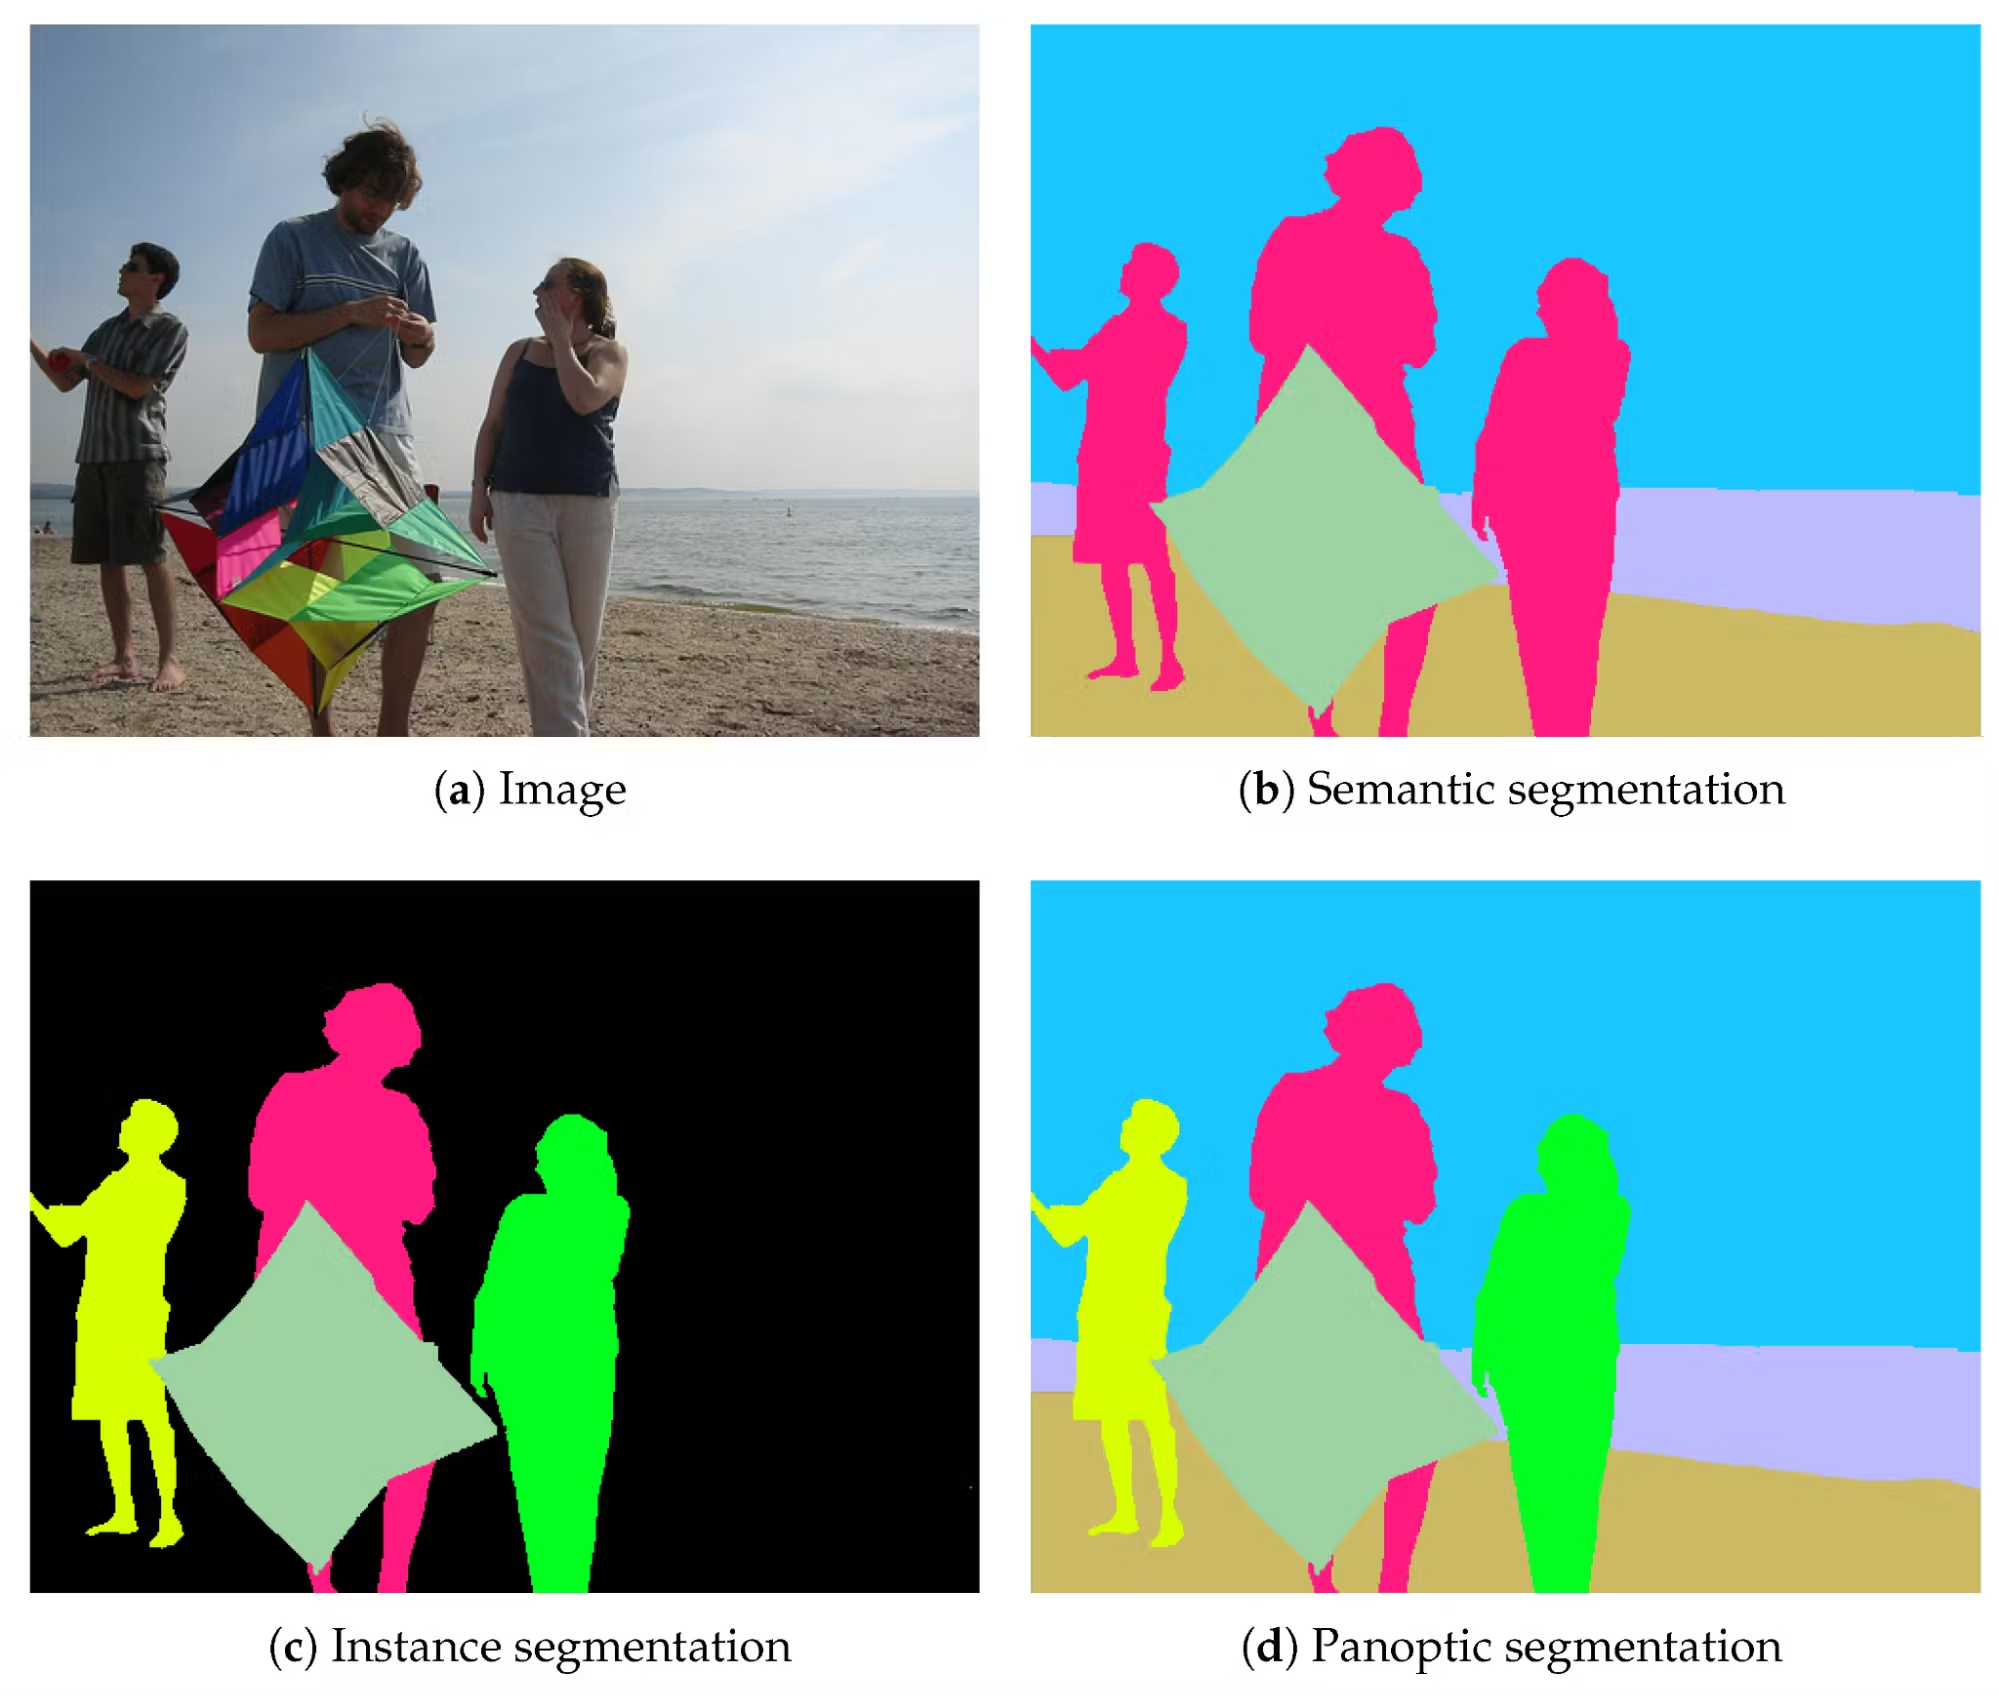
\includegraphics[scale=0.1]{images/segmentation.png}
    \caption{Different types of image segmentation}
    \label{fig:image-segmentation}
\end{figure}

Similarly to object detection, where the Intersection over Union (IoU) metric is widely adopted to evaluate the overlap between predicted and ground-truth bounding boxes, image segmentation relies on pixel-level overlap metrics.
\\
The most commonly used metric is the \textbf{Intersection over Union (IoU)}, also referred to as the \emph{Jaccard Index}. In the context of segmentation, IoU is computed as:

\begin{equation}
IoU = \frac{TP}{TP + FP + FN}
\end{equation}
where:
\begin{itemize}
    \item $TP$ (True Positives) represents the number of correctly predicted pixels belonging to a given class,
    \item $FP$ (False Positives) represents the number of pixels incorrectly assigned to that class,
    \item $FN$ (False Negatives) represents the number of pixels belonging to the class that were not correctly predicted.
\end{itemize}
Another commonly used metric is the \textbf{Dice Coefficient}, also known as the segmentation F1-score, defined as:

\begin{equation}
Dice = \frac{2TP}{2TP + FP + FN}
\end{equation}
The Dice coefficient is particularly popular in medical image segmentation, as it is more sensitive to small objects and class imbalance.

For instance segmentation and panoptic segmentation tasks, additional metrics such as \textbf{Average Precision (AP)} computed over mask IoU thresholds and \textbf{Panoptic Quality (PQ)} are often employed to jointly evaluate detection and segmentation performance.
These evaluation metrics provide a quantitative measure of the agreement between predicted segmentation masks and ground-truth annotations, enabling objective comparison between different models and approaches.